\section{$Re_{\tau}=1000$ simulation} 
The second simulation performed is carried out at $Re_{\tau}=1000$, which in terms of channel width and bulk velocity is equivalent to $Re_{b}=...$.\par
Such velocity, obtained as shown in the previous chapter, is ..., while $\alpha_{0}$ and $\beta_{0}$ are respectively 0.5 and 1, for the reasons shown before.\par
The timestep is once again constant, with \emph{dt}=0.0001 and the simulation time is T=5. \par
The simulation time is smaller than before for costing reasons, however, in order to guarantee good results, we sampled the field every 0.05 steps, so that we can employ a 100 fields to do the ensemble average.\\~\par
The grid employed in this simulation face 500 points in the wall-normal direction, 2048 in the spanwise direction and 2048 points along the streamwise dimension, direction in which we exploit the Hermitian symmetry. According to this configuration, the grid size reach the billion of points.\\~\par
Table~\ref{table:1000} report a summary of the simulation configuration for the $Re_{\tau}=1000$ case.

\begin{table}[h]
\caption{Simulation data for $Re_{\tau}$=1000}
\begin{center}
\begin{tabular}{ccccccccccccc}
\toprule
$L_{x}$ & $L_{z}$ & $\delta$ & $nx$ & $nz$ & $ny$ & $\alpha_{0}$ & $\beta_{0}$ & $\Delta x^{+}$ & $\Delta z^{+}$ & $px$ & $dt$ & $T$\\
$4\pi$ & $2\pi$ & 1 & 2048 & 2048 & 500 & 0.5 & 1 & tbd  & tbd & 1 & 0.0001 & 5 \\
\bottomrule
\end{tabular}
\end{center}
\label{table:1000}
\end{table}

Since are required approximately 40GB of disk space per each field we decided to avoid to save on disk them, instead we calculated the statistics runtime, merging the files at the end of the simulation, reducing the required space to few MB.\\~\par

Let us focus now on the statistics gained from the simulation.\par
Figure~\ref{log law:1000} report the law of the wall. As we can see from the plot, made in semi-logarithmic scale using the wall units, ...TODO \par
Far from the wall, the velocity defect law find good feedback with our results, as shown by the graph~\ref{velocity:defect:1000}.\\~\par


In figure~\ref{budget:1000} we reported the \emph{rms} fluctuations, jointed with the TKE distribution. PEAKs?? \\~\par

\begin{figure}
\begin{center}
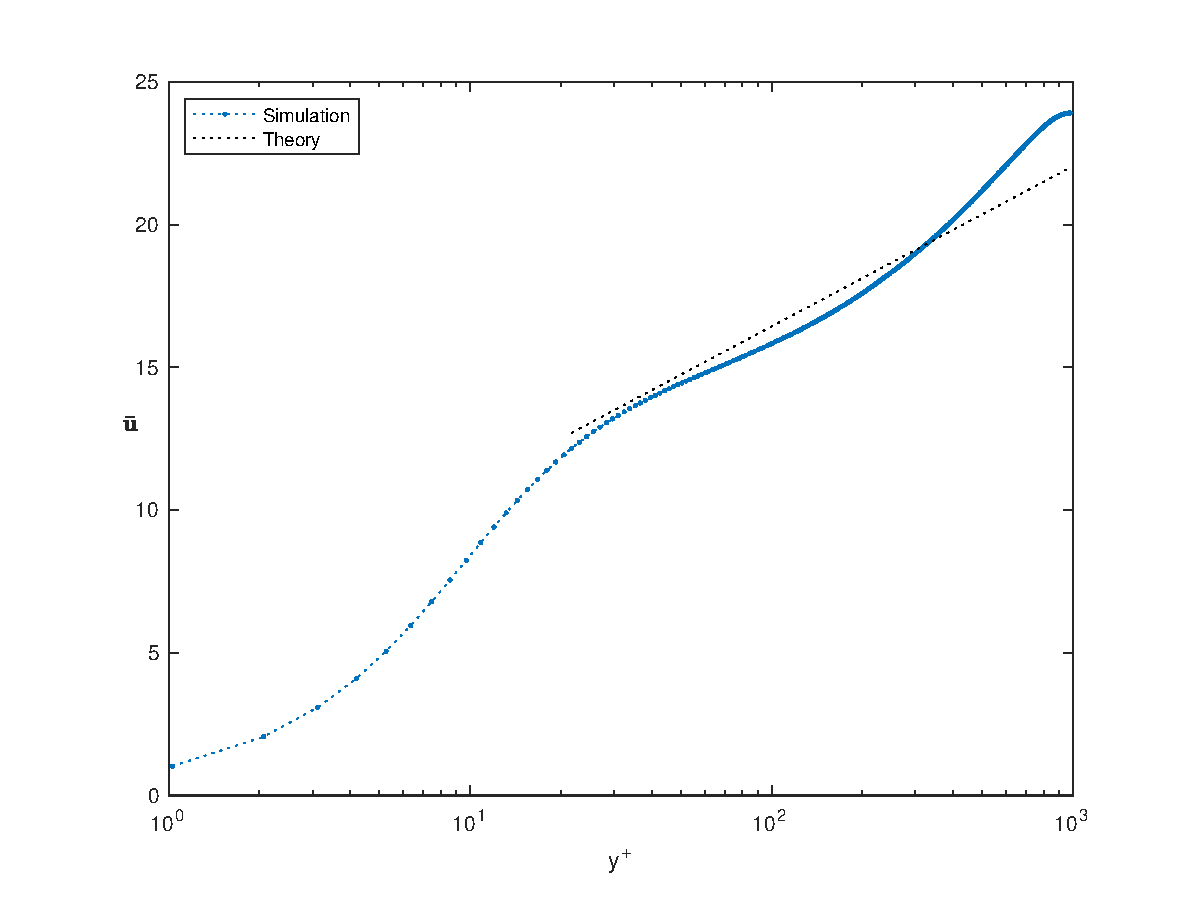
\includegraphics[scale=0.55]{grafici/loglaw_1000.eps}
\caption{$\bar{u}^{+}$ in the near wall region for a $Re_{\tau}=1000$ simulation}
\label{loglaw:1000}
\end{center} 
\end{figure}

\begin{figure}
\begin{center}
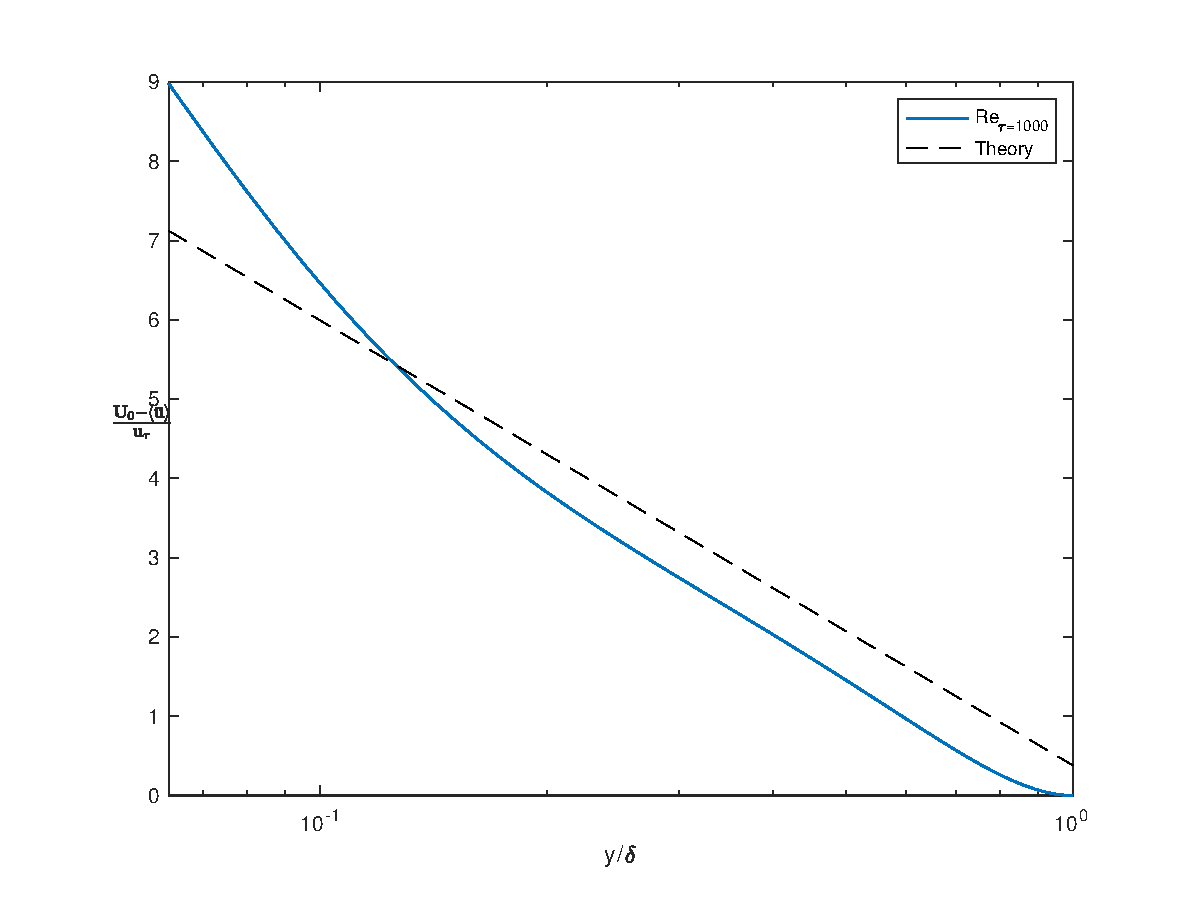
\includegraphics[scale=0.55]{grafici/velocity_defect_1000.eps}
\caption{Velocity defect for a $Re_{\tau}=1000$ simulation}
\label{velocity:defect:1000}
\end{center} 
\end{figure}

\begin{figure}
\begin{center}
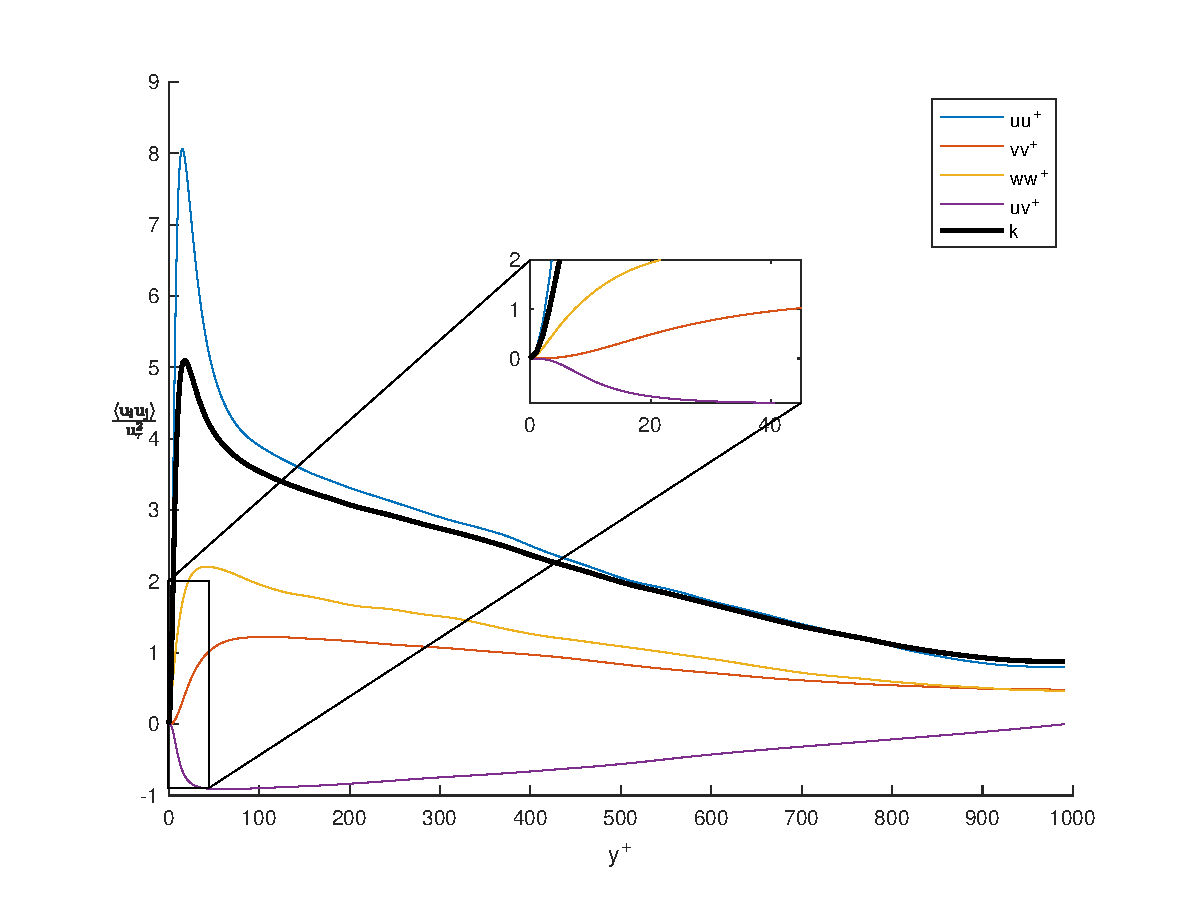
\includegraphics[scale=0.55]{grafici/budget+k_1000.eps}
\caption{\emph{rms} terms for a $Re_{\tau}=1000$ simulation}
\label{budget:1000}
\end{center} 
\end{figure}


The finer mesh and the higher Reynolds evidenced the appearance of a new turbulence peak, detached from the wall-cycle, with a less prominent peak than the latter ones. The presence of this peak can be recovered by looking at figures~\ref{rms:1000} and~\ref{tke:prod:1000}, which report the \emph{rms} terms and the turbulent kinetic energy distribution, expressed in function of the wall units, and the production term of the TKE equation.  

\begin{figure}
\begin{center}
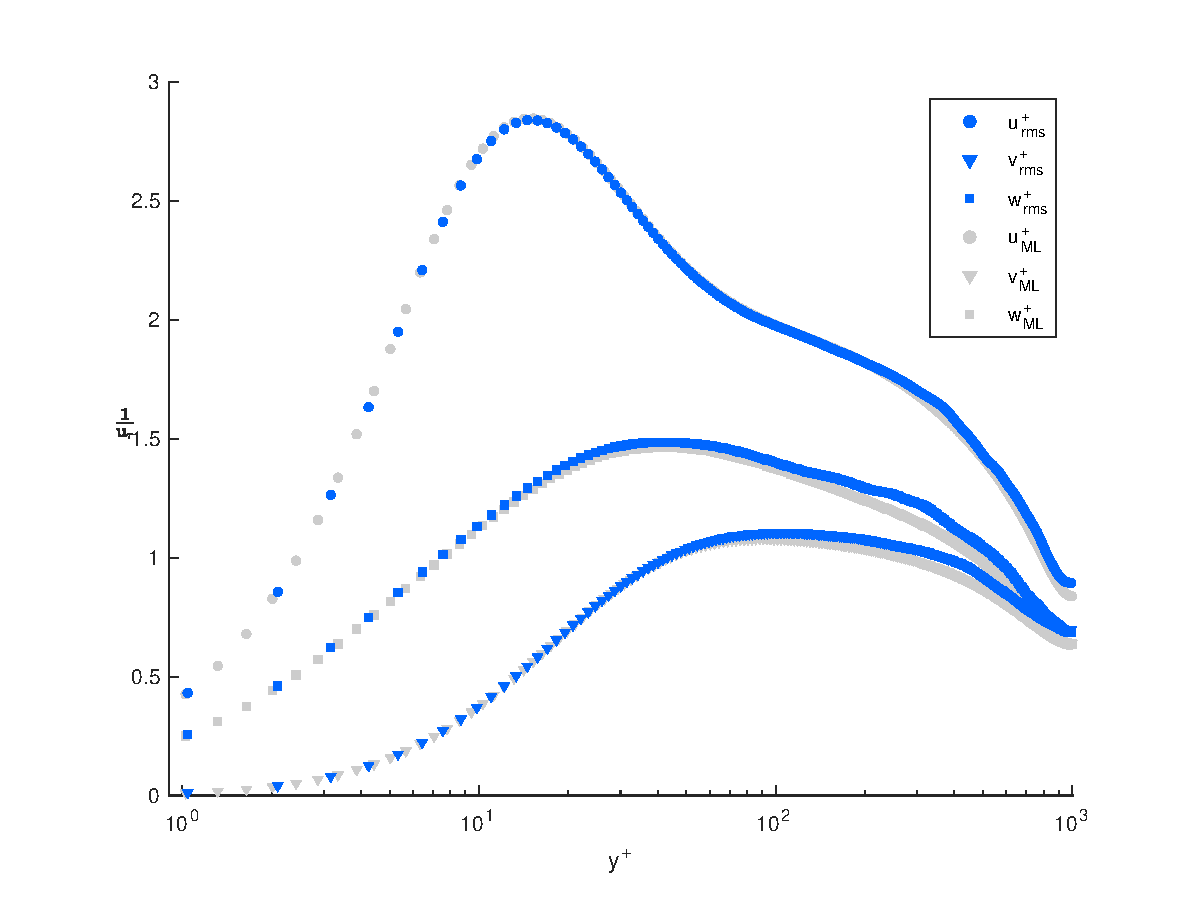
\includegraphics[scale=0.55]{grafici/rms_1000.eps}
\caption{\emph{rms} behavior on a $Re_{\tau}=1000$ simulation}
\label{rms:1000}
\end{center} 
\end{figure}

\begin{figure}
\begin{center}
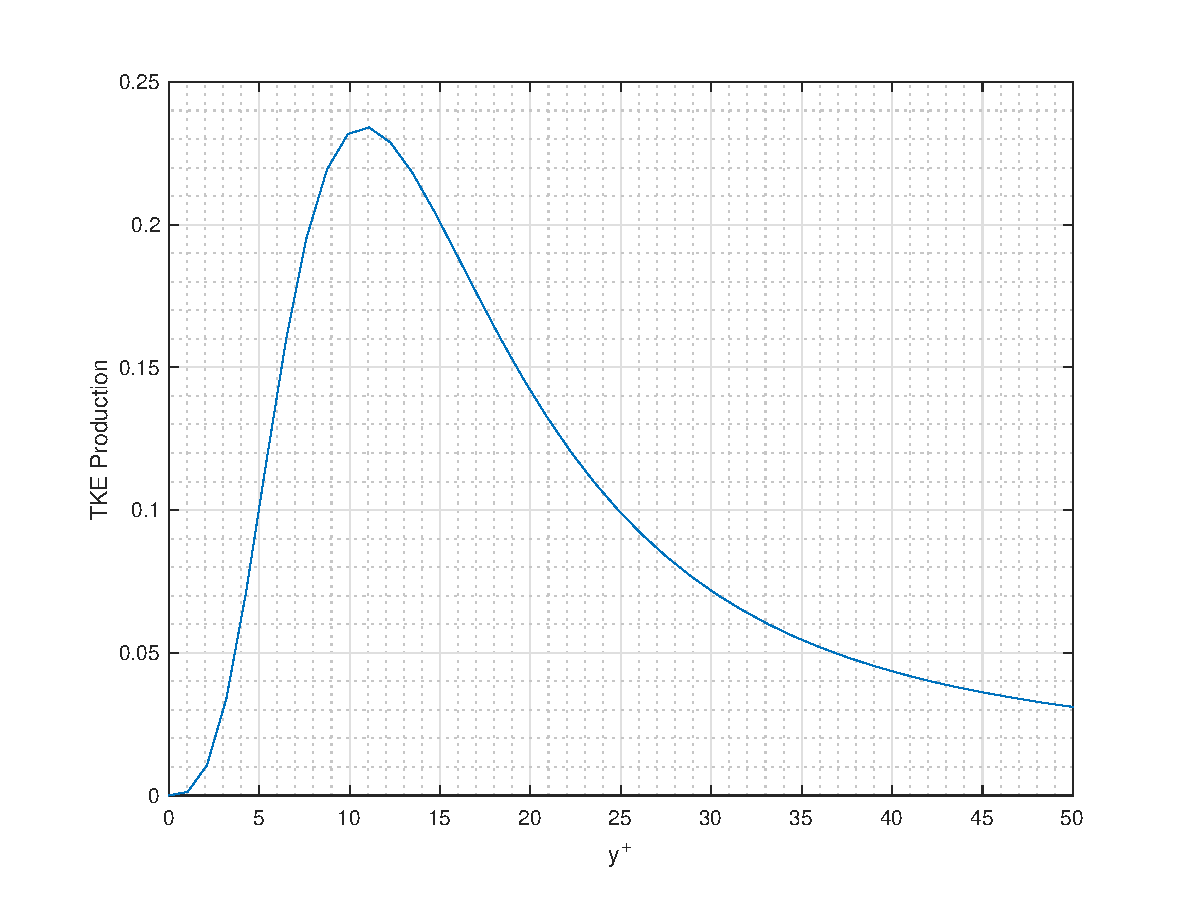
\includegraphics[scale=0.55]{grafici/tke_prod_1000.eps}
\caption{Production term of the TKE eq. for a $Re_{\tau}=1000$ simulation}
\label{tke:prod:1000}
\end{center} 
\end{figure}